\subsubsection{Statistiken}
% Das ist ein Unterpunkt von Logging
% Hier könnte man erwähnen, woraus Statistiken erstellt werden.
% Welche Lib wird verwendet? (Und warum?)
% Was werden für Statistiken erstellt?
% Wofür können sie eingesetzt werden?
%
% Und was dir sonst so einfällt.
% Hier kann man ganz viele Bilder rein tun. Die hast du wahrscheinlich eh schon alle im /images/screenshots/-Ordner
Als entscheiden wurde, dass ein umfangreiches Logging in das Projekt eingebaut wird, wurde ebenfalls entscheiden, dass diese Logs nicht ungenützt bleiben können. Um diese auszuwerten wurde auf Fremdsoftware zurückgegriffen. Mit dieser Software können Diagramm erstellt werden, mit der sehr gute Statistiken erzeugt werden können.\\
\\
Es werden verschiedenste Statistiken aus der Nutzung des Services erstellt. Die meisten Daten, zeigte sich, sind am besten in Kreisdiagramme darstellbar, weshalb in den meisten Fällen Kreisdiagramme verwendet wurden. Für das Diagramm der Seitenaufrufe wurde zum einen ein Balkendiagramm und zum anderen ein normales Liniendiagramm verwendet. Der Vorteil vom Diagramm für die täglichen Nutzungen ist, dass es die Möglichkeit bietet, im Diagramm zu zoomen. Dies ermöglicht, auch über einen großen Zeitraum, die Daten im Blick zu behalten.\\
Um die Daten nicht wesentlich zu verfälschen wurde das Entwicklungsteam nicht mitgezählt, da sonst nicht viel über die Diagramme ausgesagt werden kann.\\
Als zusätzliches Tool konnten die Statistiken der Android App verwendet werden, denn Google liefert in seiner Development Konsole viele informative Information über Downloadzahlen, Geräte, usw..\\
Um auch über die anderen Mobile-Betriebssysteme eine Aussage treffen zu können, wie viele Geräte die Apps heruntergeladen haben, wurde auch auf die Auswertung der Logs mit dem Kommandozeilen-Tool für MySQL zurückgegriffen.
\paragraph{\textit{jqPlot}\\}
jqPlot ist eine Open Source Software, welche auf der Webseite \url{http://www.jqplot.com} heruntergeladen werden kann. Das heruntergeladene Archiv muss entpackt werden und kann anschließend auf den Webserver kopiert werden. Diese Paket ist sehr umfangreich. Es können viele verscheidene Diagramme erstellt werden und ist einfach zu integrieren. Die Dokumentation zu dieser Software ist unter der Webseite \url{http://www.jqplot.com/docs/files/usage-txt.html} zu finden und ist sehr umfangreich. Durch die gute Dokumentation und durch die Erfahrung vor der Diplomarbeit mit dieser Software, wurde beschlossen diese Software zu verwenden.
\subsubsection{Erkenntnisse} \label{sec:content_draft_log_erkenn}
% Hier kann man aktuelle Werte erwähnen und diskutieren (in Bezug auf Uhrzeiten, Wochenende, Geräte, etc).
%
% Vielleicht hier dazu schreiben, dass das zwar interessant ist, allerdings für das Projekt selbst eher unwichtig ist, wir wollten es aber trotzdem erwähnen. #oderso#
Nach dem Öffnen von SIS für die N-Abteilung überprüften wir immer wieder die Statistiken, um über die Popularität unseres Services immer auf dem neusten Stand zu sein. Im Laufe der, nun schon 2 Monat andauernden, Testphase, konnten wir interessante Ergebnisse über die Verwendung unseres Services in Erfahrung bringen. Im folgendem werden einige interessante Ergebnisse dargestellt.(Stand 28.04.2014)\\

\paragraph{App\\}
Die App wurde für die 3 bekanntesten Plattformen entwickelt. Diese sind Android, iOS und Windows Phone. Die Auswertung der Diagramme ist nicht ganz korrekt, da die Apps in großen Zeitabständen nacheinander in Umlauf gebracht wurden, daraus ergibt sich für manche Apps einen gewissen Vorsprung. Jedoch kann ein wenig auf die Nutzung und die Masse der einzelnen Geräte zurück geschlossen werden, wenn man beachtet wie schnell eine Plattform eine Andere überholt hat.\\
In diesem Zusammenhang kann man iOS nennen, da diese App sehr spät verteilt werden konnte, jedoch schon nach ca. 1 Woche die Windows Phone App, gemessen an den Seitenaufrufen, überholt hat. Momentan liegt die iOS App deutlich vor der Windows Phone App. Wie schon erwartet liegt Android weit abgeschlagen vorne. (siehe \autoref{fig:content_draft_log_app})\\
Nach einer Auswertung der Logs im Kommandozeilen-Tool konnte der Grund für diese Aufteilung sofort gefunden werden. Dabei stellte sich heraus, dass es insgesamt 8 Windows Phone User gibt, davon 3 Lehrer und 5 Schüler. Das erklärt natürlich, dass 61 iOS User die 8 Windows Phone User sofort überholen konnten. Erstaunlich ist, dass es nur 2 Lehrer gibt, die das iOS App verwenden. Android ist mit insgesamt 203 User weit abgeschlagen, von diesen 203 User haben sich 12 Lehrer die App heruntergeladen. Verglichen mit den Zahlen, dass unser Service von insgesamt 19 Lehrern verwendet wird, heißt das, dass von 19 Lehrern 17 Lehrer die App verwenden. Insgesamt haben sich 290 Schüler an unserem Service angemeldet, das bedeutet verglichen mit der App, dass davon ca. 93 \% der Schüler die App verwenden. 
\begin{figure}[H]
\centering
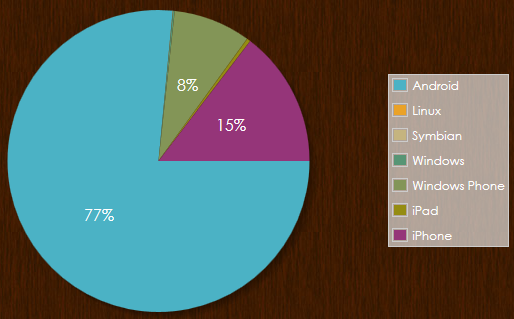
\includegraphics[keepaspectratio=true, width=12cm]{images/screenshots/statistics/app_plattform.png}
\caption{Plattform-App}
\label{fig:content_draft_log_app}
\end{figure}

In der Development Console von Google kann genau eingesehen werden, wann, welches Gerät, welche Android-Version, Land und Sprache die App installiert und deinstalliert hat. Somit ergaben sich die Zahlen, dass unsere App von 120 Personen heruntergeladen und davon haben sie momentan 91 Personen noch auf ihrem Gerät installiert. Die relativ große Differenz lässt sich dahingehend erklären, dass die App wahrscheinlich auch von Personen heruntergeladen wurde, welche die App nicht betrifft. Außerdem ist unsere App 20 mal bewertet worden und hat eine durchschnittliche Bewertung von 4,85 von maximalen 5 Punkten. In der \autoref{fig:content_draft_log_app_install} ist die Statistik zu sehen, wann die App installiert worden ist.

\begin{figure}[H]
\centering
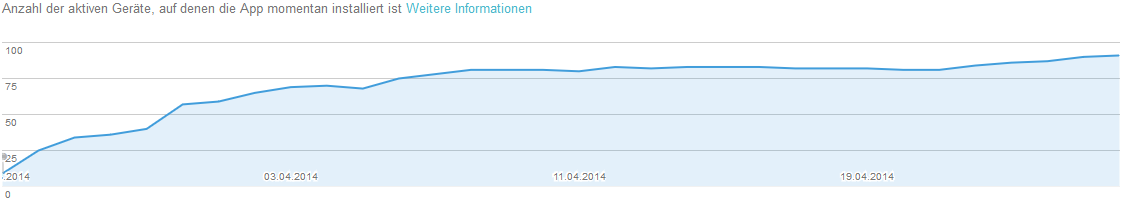
\includegraphics[keepaspectratio=true, width=17cm]{images/screenshots/statistics/app_install.png}
\caption{Plattform-App}
\label{fig:content_draft_log_app_install}
\end{figure}

\paragraph{PC\\}
Wie auch schon bei der App gibt es, wie erwartet, auch bei den PC Plattformen einen, weit abgeschlagenen, ersten Platz, was die Nutzung anbelangt. Dies ist natürlich Windows. In der \autoref{fig:content_draft_log_pc} ist zu sehen, dass sich eigentlich keine andere Plattform mit Windows messen kann. In der \autoref{fig:content_draft_log_pc} sind auch viele Mobile Betriebssysteme zu sehen, dies kann darauf zurückzuführen sein, dass viele dieser Geräte die Webseite besucht haben, dadurch werden sie auch in dieser Statistik gezählt. Diese Mobilen Geräte werden, bevor es die App gab, die Webseite benützt haben. Erstaunlich ist, dass Mac OSX vor Linux liegt.
\begin{figure}[H]
\centering
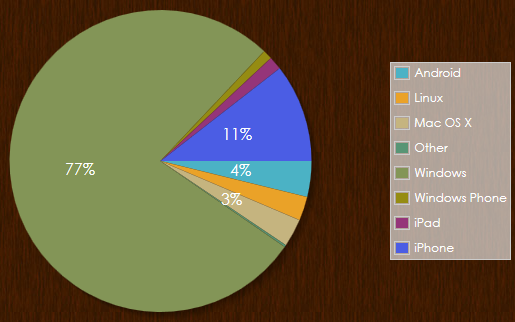
\includegraphics[keepaspectratio=true, width=12cm]{images/screenshots/statistics/pc_plattform.png}
\caption{Plattform-PC}
\label{fig:content_draft_log_pc}
\end{figure}

Firefox ist bei den Browsern auf unserer Webseite am meisten vertreten. Neben Firefox ist auch noch Safari Internet Explorer und Chrome zu nennen. Die sich die restlichen ca. 50 \% teilen. (siehe \autoref{fig:content_draft_log_pc_browser})

\begin{figure}[H]
\centering
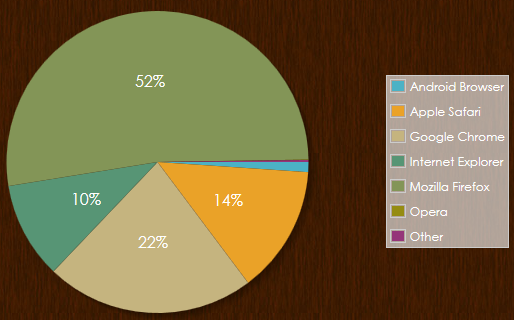
\includegraphics[keepaspectratio=true, width=12cm]{images/screenshots/statistics/pc_browser.png}
\caption{Browser-PC}
\label{fig:content_draft_log_pc_browser}
\end{figure}

\paragraph{App/PC\\}
Eine der interessantesten Statistik ist die Aufteilung der Seitenaufrufe zwischen App und PC. Wenn man bedenkt, dass die App wesentlich später den breiten Massen vorgeführt wurde, ist die App bei weitem attraktiver bei den Nutzern als der PC. Anfangs war die App dem PC unterlegen, als aber die App für Android und Windows Phone in Umlauf kam, holte die App immer weiter auf. Momentan liegt die App be 63 \% und der PC bei 37 \%. Die Tendenz der App zeigt jedoch nach oben. Vielleicht lässt sich dieses Phänomen auch daran erklären, dass man aus Langeweile eher kurz die App aufmacht die einzelnen Punkte durchsieht und sie wieder schließt, dies ist im Web nicht so leicht möglich. Deshalb sieht es im Moment so aus, dass die App, auf lange Sicht gesehen, das Web verdrängen wird.

\paragraph{Zugriffszeiten\\}
Interessant sind auch die Zugriffszeiten und die Anzahl der Seitenaufrufe pro Tag.\\
Mit diesen Diagrammen kann man die Zeiten herausfinden, an denen der Service am häufigsten genutzt wird. Das Ergebnis liefert, dass im Durchschnitt die Nutzung unseres Services um 7 Uhr beginnt und um 22 Uhr endet. In dieser Zeit kann man sehen, dass zwischen 7 und 8 Uhr die meisten Aufrufe getätigt werden. Dies nimmt dann stetig ab, bis zwischen 9 und 10 Uhr noch ein Maximum erreicht wird. Im Laufe des Tages nehmen die Aufrufe leicht ab, bis sie zwischen 16 und 17 Uhr ihr Minimum erreichen. Zwischen 12 und 13 Uhr ist nochmals eine Erhöhung zu sehen. Ab 17 Uhr steigen die Zahlen wieder und erreichen zwischen 21 - 22 Uhr das Maximum. (siehe \autoref{fig:content_draft_log_zugriff_std})

\begin{figure}[H]
\centering
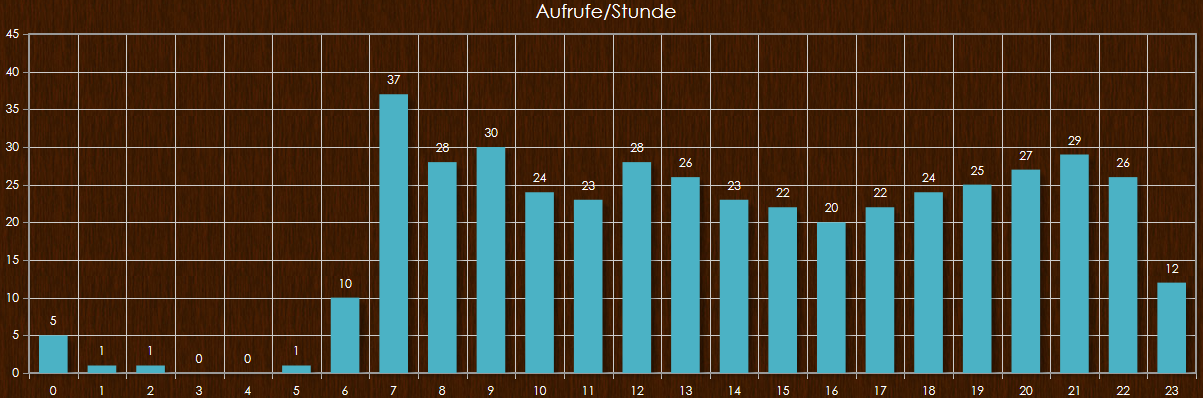
\includegraphics[keepaspectratio=true, width=17cm]{images/screenshots/statistics/aufruf_std.png}
\caption{Aufrufe/Stunde}
\label{fig:content_draft_log_zugriff_std}
\end{figure}

Wird der Zeitraum von einer Woche betrachtet, dann ist zu sehen, dass die Aufrufe während einer Woche sehr schwanken, sie sind jedoch jeden Tag in einem Bereich, wo man sagen kann, dass unser Service gut genutzt wird. Am Samstag kann beobachtet werden, dass am wenigsten Aufrufe zusammen kommen. Am Sonntag beginnen die Nutzer wieder den Service zu nutzen, dies sieht man an den steigenden Aufrufszahlen. Es konnte beobachtet werden, dass es immer wieder während den Wochentagen ein Ausreißer nach oben gibt, es konnte jedoch kein Muster erkannt werden. (siehe \autoref{fig:content_draft_log_zugriff_tag})


\begin{figure}[H]
\centering
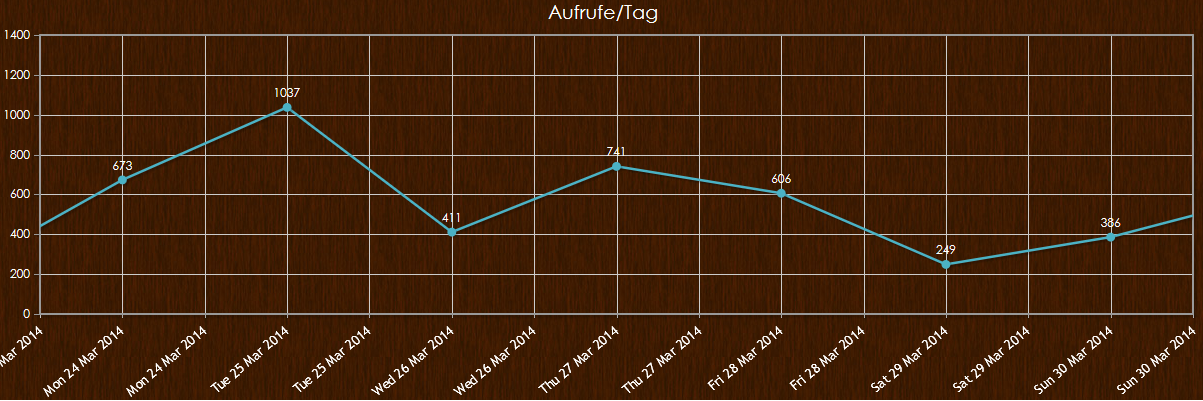
\includegraphics[keepaspectratio=true, width=17cm]{images/screenshots/statistics/aufruf_tag.png}
\caption{Aufrufe/Tag}
\label{fig:content_draft_log_zugriff_tag}
\end{figure}

\paragraph{Jahrgänge und Lehrer\\}
Ein sehr auffallendes Muster konnte bei der Aufteilung, von der Nutzung der einzelnen Jahrgängen und Lehrer, erkannt werden. Erstaunlich ist, dass der erste Jahrgang unseren Service wesentlich mehr nutzt, als alle anderen Jahrgänge. Außerdem nimmt die Nutzung unseres Services mit steigendem Jahrgang ab. Dies kann auf die sinkende Schülerzahl der Jahrgänge nach oben hin in Verbindung gebracht werden oder es kommt daher, dass die jüngere Generation öfters auf ihr Smartphone schaut oder im Web unterwegs ist.\\
Nach dem 1. Jahrgang kommen die Lehrer von der Nutzungshäufigkeit gesehen, dies ist wahrscheinlich darauf zurückzuführen, dass die Administratoren Lehrer sind und deshalb unseren Service wesentlich öfters nutzen. (siehe \autoref{fig:content_draft_log_jahr})

\begin{figure}[H]
\centering
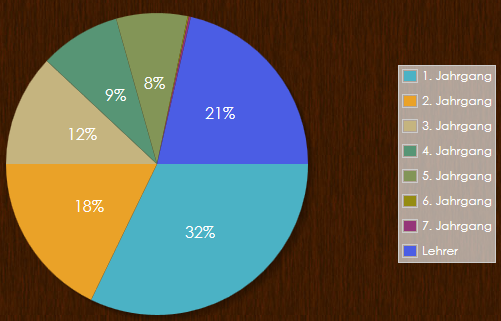
\includegraphics[keepaspectratio=true, width=12cm]{images/screenshots/statistics/jahrgang.png}
\caption{Aufrufe/Tag}
\label{fig:content_draft_log_jahr}
\end{figure}